% Created 2016-08-17 Wed 14:38
\documentclass[tikz]{standalone}

\usepackage[utf8]{inputenc}
\usepackage[T1]{fontenc}

\usepackage{circledsteps}

\RequirePackage{xcolor}

%% HPI color definitions according to the design manual
% These do not exactly match the RGB values used in the Powerpoint slide master due to unknown reasons
\definecolor{hpiyellow}{RGB}{246,168,0}
\definecolor{hpiorange}{RGB}{221,97,8}
\definecolor{hpired}{RGB}{177,6,58}
\definecolor{hpigray}{RGB}{90,96,101}
\definecolor{hpiblue}{RGB}{0,122,158}


\renewcommand{\sfdefault}{neosans}
% Different font weights for neosans
\newcommand{\textl}[1]{{\fontseries{l}\selectfont #1}} % light
\newcommand{\textm}[1]{{\fontseries{m}\selectfont #1}} % medium, same as default weight
\newcommand{\textsb}[1]{{\fontseries{sb}\selectfont #1}} % semibold
\newcommand{\textmb}[1]{{\fontseries{mb}\selectfont #1}} % bold, same as \textbf
\newcommand{\texteb}[1]{{\fontseries{eb}\selectfont #1}} % extra bold
\newcommand{\textub}[1]{{\fontseries{ub}\selectfont #1}} % ultra bold

\tikzset{every picture/.style={/utils/exec={\sffamily}}}
\tikzset{flipflop RSflanke/.style={
  flipflop,
  flipflop def={t1=S, t2=C, c2=1, t3=R, t6=Q, t4={\ctikztextnot{Q}}}
}}


\tikzset{
  mechanicalSwitch/.pic={
    \coordinate (-inUp) at (135:2); 
    \coordinate (-inDown) at (235:2);
    \coordinate (-out) at (2,0);
    \coordinate (-center) at (0,0);
    
    \draw (0,0) circle [radius = 2cm];
    \draw [fill=gray!20] (0,0) circle [radius = 0.2cm];

    \draw (0, 0) -- (2, 0);
    \draw (135:.8) -- (135:2); 
    \draw (225:.8) -- (225:2); 

    \draw [fill=gray!20] (2, 0) circle [radius=0.05cm]; 
    \draw [fill=gray!20] (135:2) circle [radius=0.05cm]; 
    \draw [fill=gray!20] (225:2) circle [radius=0.05cm]; 

    
    \draw [thick] (0,0) -- (175:1.5); 

    \draw [dashed, <->, domain=135:225] plot ({cos(\x)}, {sin(\x)}); 
  },
  mechanicalSwitchClosed/.pic={
    \coordinate (-inUp) at (135:2); 
    \coordinate (-inDown) at (255:2);
    \coordinate (-out) at (2,0);
    \coordinate (-center) at (0,0);
    \draw (0,0) circle [radius = 2cm];
    \draw [fill=gray!20] (0,0) circle [radius = 0.2cm];

    \draw (0, 0) -- (2, 0);
    \draw (135:.8) -- (135:2); 
    \draw (225:.8) -- (225:2); 

    \draw [fill=gray!20] (2, 0) circle [radius=0.05cm]; 
    \draw [fill=gray!20] (135:2) circle [radius=0.05cm]; 
    \draw [fill=gray!20] (225:2) circle [radius=0.05cm]; 

    
    \draw [thick] (0,0) -- (135:2); 

    \draw [dashed, <->, domain=135:225] plot ({cos(\x)}, {sin(\x)}); 
  }
}


\usetikzlibrary{calc}
\usetikzlibrary{positioning}



\usepackage{pgfplots}

\begin{document}

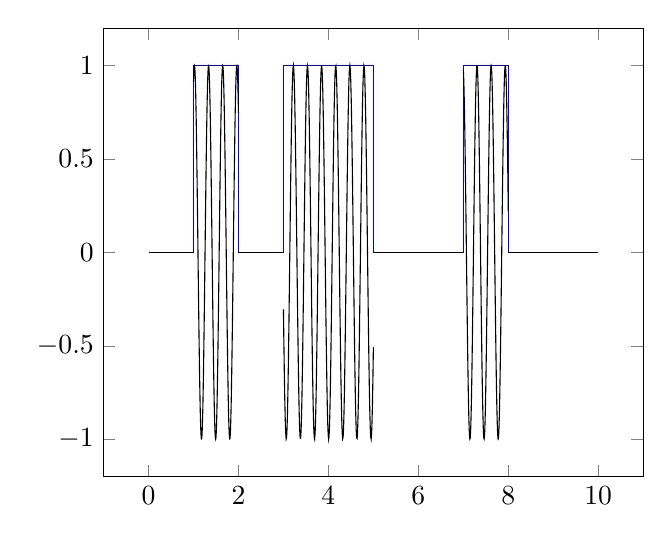
\begin{tikzpicture}
  \label{page:phy:xonxoff}
  \begin{axis}
    [no markers,
    % samples=500,
    domain=0:10,
    trig format plots=rad,    
    ]
    \addplot coordinates {(0,0) (1,0) (1,1) (2,1) (2,0) (3,0) (3,1) (5,1) (5,0) (7,0) (7,1) (8,1) (8,0) (10,0)};

    \addplot [domain=0:1] expression { 0}; 
    \addplot [domain=1:2, samples=200] expression { 1*sin(20*x) }; 
    \addplot [domain=2:3] expression { 0}; 
    \addplot [domain=3:5, samples=200] expression { 1*sin(20*x) }; 
    \addplot [domain=5:7] expression { 0}; 
    \addplot [domain=7:8, samples=200] expression { 1*sin(20*x) }; 
    \addplot [domain=8:10] expression { 0}; 

  \end{axis}

\end{tikzpicture}


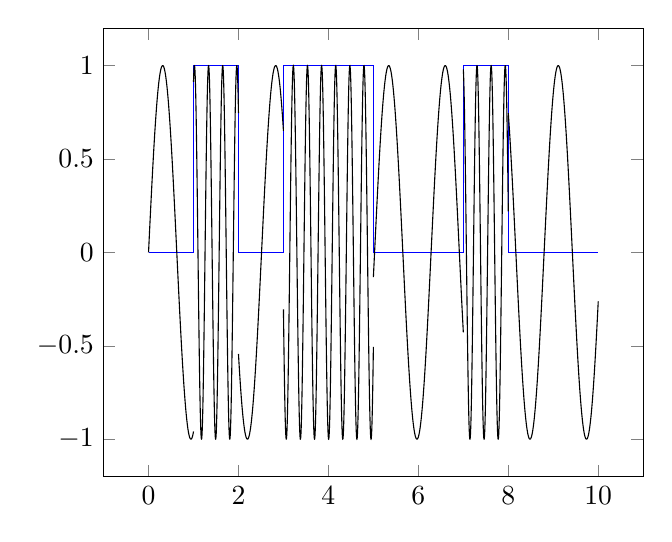
\begin{tikzpicture}
  \label{page:phy:freqmod}

  \begin{axis}
    [no markers,
    samples=1000,
    domain=0:10,
    trig format plots=rad,    
    ]
    \addplot coordinates {(0,0) (1,0) (1,1) (2,1) (2,0) (3,0) (3,1) (5,1) (5,0) (7,0) (7,1) (8,1) (8,0) (10,0)};

    \addplot [domain=0:1] expression { 1*sin(5*x) }; 
    \addplot [domain=1:2] expression { 1*sin(20*x) }; 
    \addplot [domain=2:3] expression { 1*sin(5*x) }; 
    \addplot [domain=3:5] expression { 1*sin(20*x) }; 
    \addplot [domain=5:7] expression { 1*sin(5*x) }; 
    \addplot [domain=7:8] expression { 1*sin(20*x) }; 
    \addplot [domain=8:10] expression { 1*sin(5*x) }; 

  \end{axis}

\end{tikzpicture}


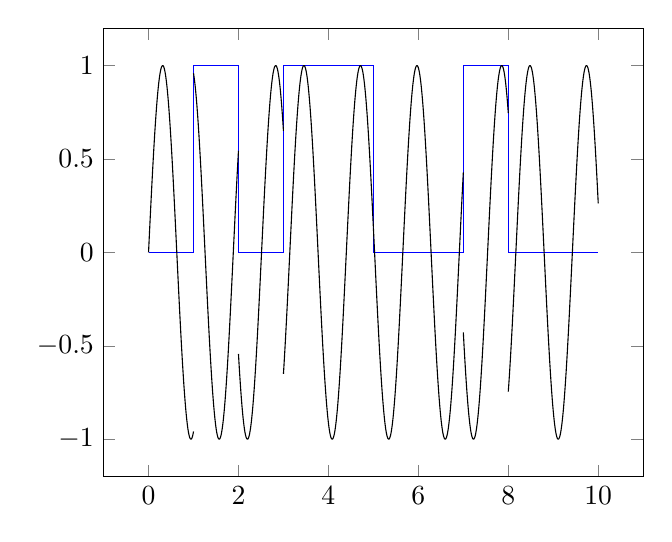
\begin{tikzpicture}
  \label{page:phy:phasemod}

  \begin{axis}
    [no markers,
    samples=1000,
    domain=0:10,
    trig format plots=rad,    
    ]
    \addplot coordinates {(0,0) (1,0) (1,1) (2,1) (2,0) (3,0) (3,1) (5,1) (5,0) (7,0) (7,1) (8,1) (8,0) (10,0)};

    \addplot [domain=0:1] expression { 1*sin(5*x) }; 
    \addplot [domain=1:2] expression { 1*sin(5*x + pi) }; 
    \addplot [domain=2:3] expression { 1*sin(5*x) }; 
    \addplot [domain=3:5] expression { 1*sin(5*x + pi) }; 
    \addplot [domain=5:7] expression { 1*sin(5*x + pi) }; 
    \addplot [domain=7:8] expression { 1*sin(5*x) }; 
    \addplot [domain=8:10] expression { 1*sin(5*x + pi) }; 

  \end{axis}

\end{tikzpicture}


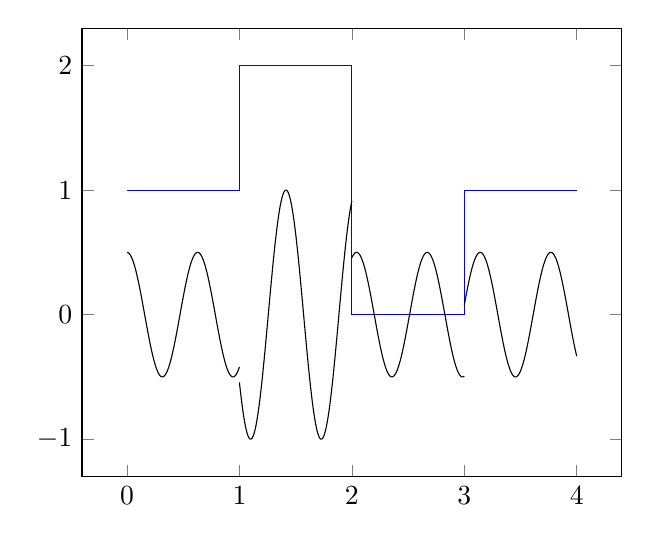
\begin{tikzpicture}
  \label{page:phy:qpsk}

  \begin{axis}
    [no markers,
    samples=1000,
    domain=0:10,
    trig format plots=rad,    
    ]
    \addplot coordinates { (0,1) (1,1) (1,2) (2,2) (2,0) (3,0) (3,1) (4,1)}; 

    \addplot [domain=0:1] expression { 0.5*sin(10*x +pi/2) }; 
    \addplot [domain=1:2] expression { 1*sin(10*x) }; 
    \addplot [domain=2:3] expression { 0.5*sin(10*x) }; 
    \addplot [domain=3:4] expression { 0.5*sin(10*x + pi/2) }; 

  \end{axis}

\end{tikzpicture}



% \begin{tikzpicture}
%   \begin{axis}
%     [no markers,
%     % samples=500,
%     domain=0:10,
%     trig format plots=rad,    
%     ]
%     \addplot [domain=0:1] expression { 0}; 
%     \addplot [domain=1:2, samples=200] expression { 1*sin(20*x) }; 
%     \addplot [domain=2:3] expression { 0}; 
%     \addplot [domain=3:5, samples=200] expression { 1*sin(20*x) }; 
    
%   \end{axis}
% \end{tikzpicture}



\end{document}